\section{Analisi di Sensibilità}

L'analisi di sensitività è stata condotta sul modello SEIR, 
come illustrato in Figura \ref{fig:ODE_Julia_example}. 
Questa analisi mirava a valutare come il modello reagisse a 
variazioni specifiche dei suoi parametri, le quali potrebbero 
condurre a comportamenti inattesi o peculiari.

Per effettuare l'analisi di sensitività, sono stati impiegati i 
metodi forniti dalla suite SciML.ai. Ciò ha permesso di identificare 
i parametri ai quali il modello è più sensibile.

\begin{minipage}{\linewidth}
	\centering
	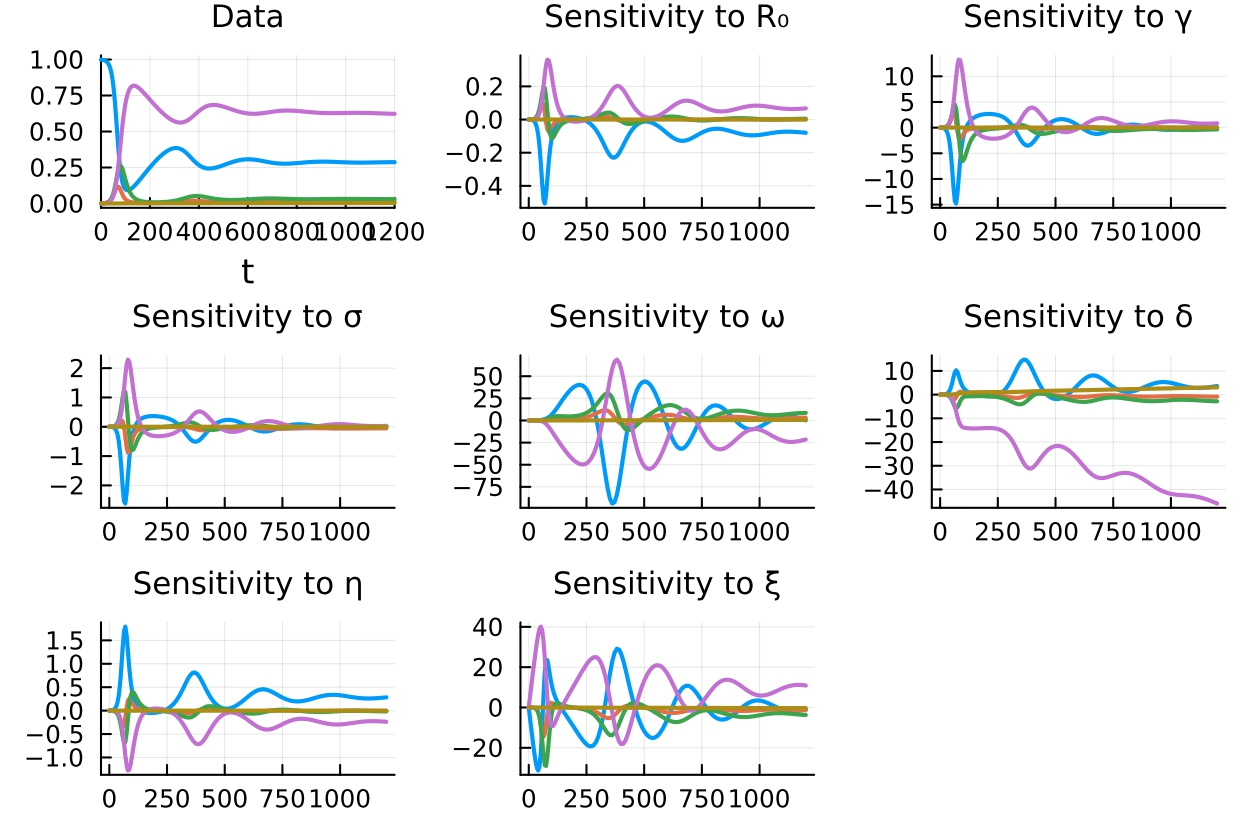
\includegraphics[width=\textwidth]{img/sa.jpg}
	\captionof{figure}{Grafico rappresentante l'analisi di sensitività del modello}
	\label{fig:sens_anal}
\end{minipage}

Come evidenziato nella Figura \ref{fig:sens_anal}, il modello 
dimostra una sensitività uniforme rispetto ai parametri 
$R_0$, $\gamma$, e $\sigma$, il che è coerente, dato che essi 
influiscono sull'andamento dell'epidemia. La sensitività ai parametri 
$\omega$ e $\delta$ era attesa, ma è risultata più marcata di 
quanto previsto. La sensitività al parametro $\eta$, che influisce 
sulle contromisure, è inversamente correlata a quella del 
parametro $R_0$, come previsto, poiché $\eta$ è direttamente 
legato alle misure di contenimento. La sensitività al parametro 
$\xi$ mostra un comportamento singolare, probabilmente dovuto 
alla sua correlazione con $\omega$, entrambi legati al compartimento 
"R" del modello, che gestisce gli individui guariti e vaccinati.

In una fase successiva dell'analisi, è stata condotta un'analisi di 
sensitività sui parametri specifici del modello ad agenti, 
utilizzando la funzione \textbf{paramscan} fornita dalla libreria 
\textbf{Agents.jl}. Sono stati individuati e selezionati quei 
parametri che potrebbero avere un notevole impatto sul comportamento 
generale del modello. Questa selezione è stata fatta in base al 
potenziale di tali parametri di innescare cambiamenti significativi nei 
risultati della simulazione.

È importante notare che alcuni parametri, specificamente quelli 
legati al controllore e alla campagna di vaccinazione, sono stati 
esclusi da questa analisi. Ciò è dovuto al fatto che variazioni in 
questi parametri possono comportare cambiamenti sostanziali nella 
simulazione, e pertanto sono stati considerati separatamente e 
successivamente analizzati in modo dettagliato.

\begin{minipage}{\linewidth}
	\centering
	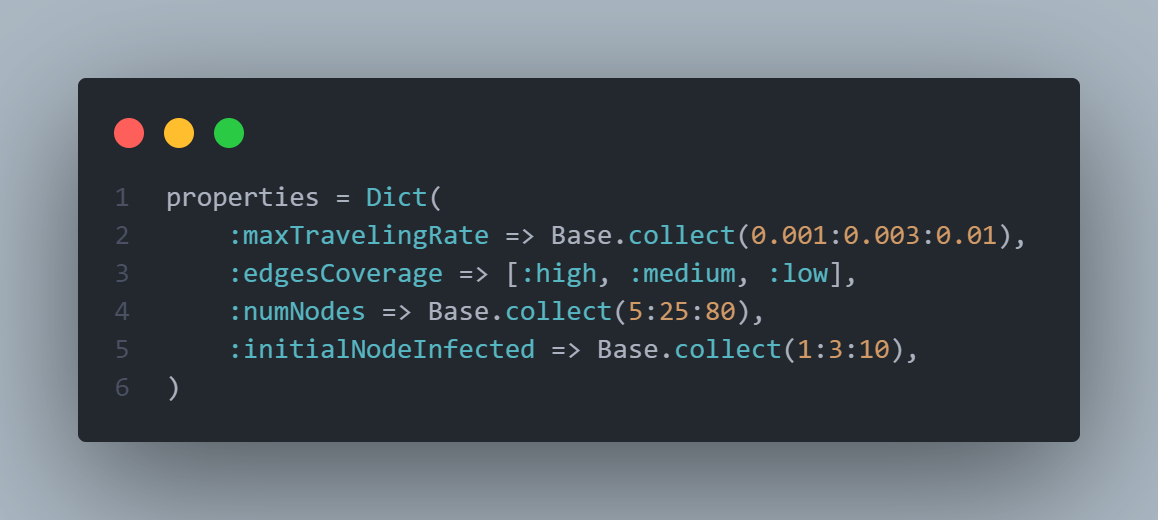
\includegraphics[width=\textwidth]{img/paramscan.png}
	\captionof{figure}{Parametri usati per l'analisi di sensitività del modello ad agente}
	\label{fig:paramscan}
\end{minipage}

L'analisi di sensitività sui parametri rimanenti mira a esplorare 
come variazioni specifiche in ciascuno di essi possano influenzare 
il comportamento complessivo del modello. Questo tipo di analisi è 
fondamentale per comprendere la sensibilità del sistema a variazioni 
nei parametri e per valutare le risposte del modello a differenti 
condizioni.

In definitiva, questa analisi di sensitività fornisce un quadro più 
completo della dinamica del modello, consentendo di identificare i 
parametri chiave che influenzano le sue prestazioni e fornendo 
indicazioni importanti per la calibrazione e l'ottimizzazione del 
modello stesso.
\newpage

\subsection{Analisi del Comportamento in Base al Numero Iniziale di Nodi Infetti}

L'analisi condotta ha investigato l'impatto del numero iniziale di 
nodi infetti sul comportamento complessivo del modello. 
I risultati hanno dimostrato che un numero maggiore di nodi infetti 
iniziali conduce a un raggiungimento più rapido del picco di infetti 
nel corso della simulazione. Tuttavia, non sono stati osservati altri 
cambiamenti significativi nel comportamento del modello.

Questo risultato era atteso e coerenza con le dinamiche epidemiologiche 
conosciute. Infatti, è noto che un aumento del numero iniziale di 
individui infetti in una popolazione può accelerare l'espansione della 
malattia e portare a un picco di infetti più precoce. 
Tuttavia, le altre dinamiche del modello, come il tasso di diffusione 
del virus, la progressione della pandemia e le misure di intervento, 
non sono state influenzate in modo significativo da questa variazione.

\begin{figure}[!hb]
	\centering
	\begin{subfigure}[b]{0.45\textwidth}
		\centering
		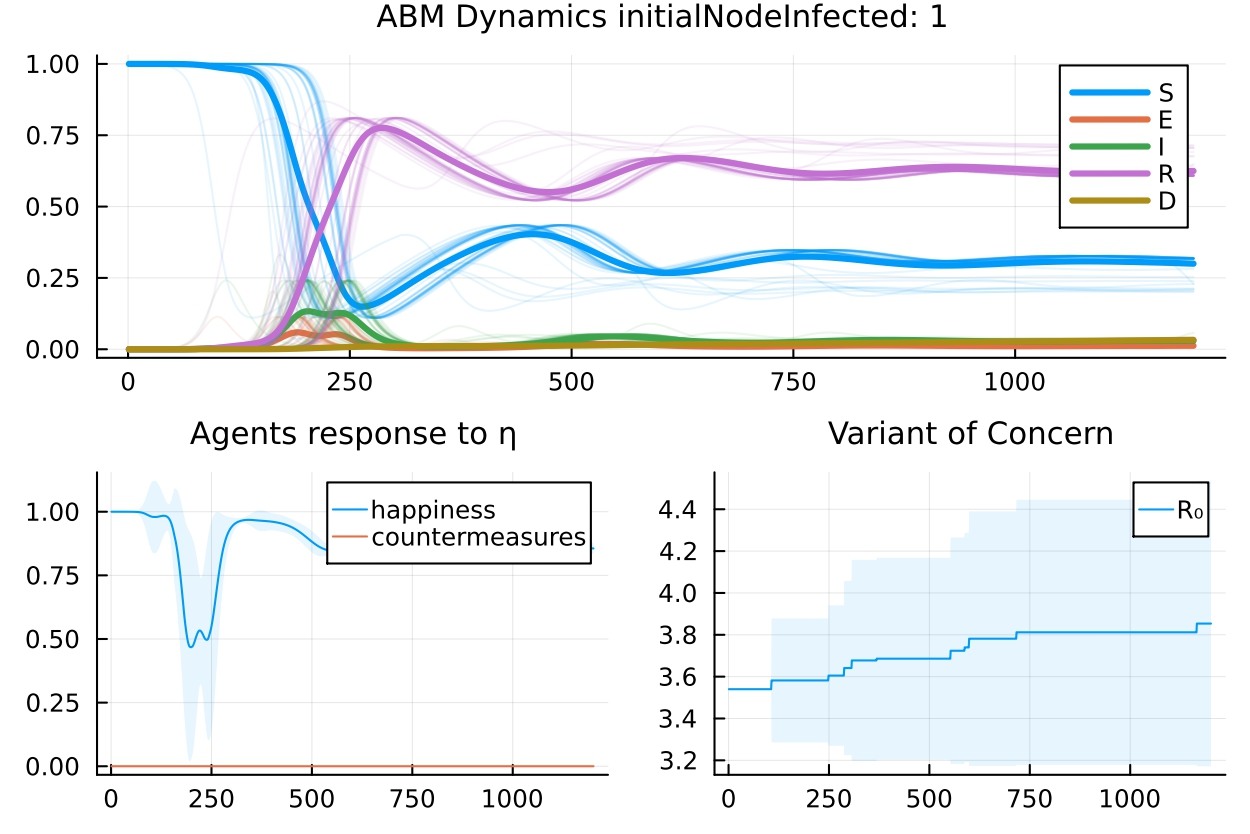
\includegraphics[width=\textwidth]{img/SocialNetworkABM_1_II.jpg}
		\caption{Grafico per la comparazione sul numero di nodi infetti di partenza. Numero nodi infetti iniziali 1}
		\label{fig:comparison_init_node_inf_1}
	\end{subfigure}
	\hfill
	\begin{subfigure}[b]{0.45\textwidth}
		\centering
		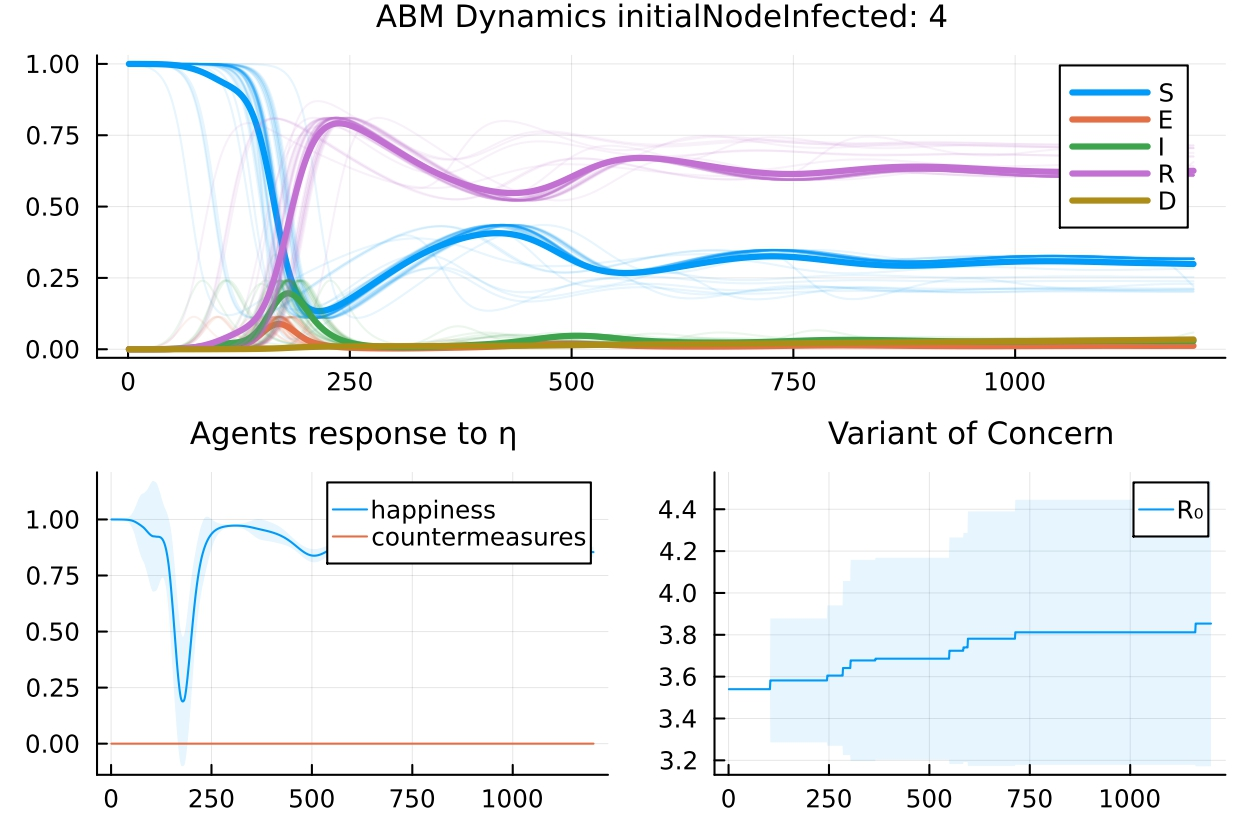
\includegraphics[width=\textwidth]{img/SocialNetworkABM_2_II.jpg}
		\caption{Grafico per la comparazione sul numero di nodi infetti di partenza. Numero nodi infetti iniziali 4}
		\label{fig:comparison_init_node_inf_4}
	\end{subfigure}
	\hfill
	\begin{subfigure}[b]{0.45\textwidth}
		\centering
		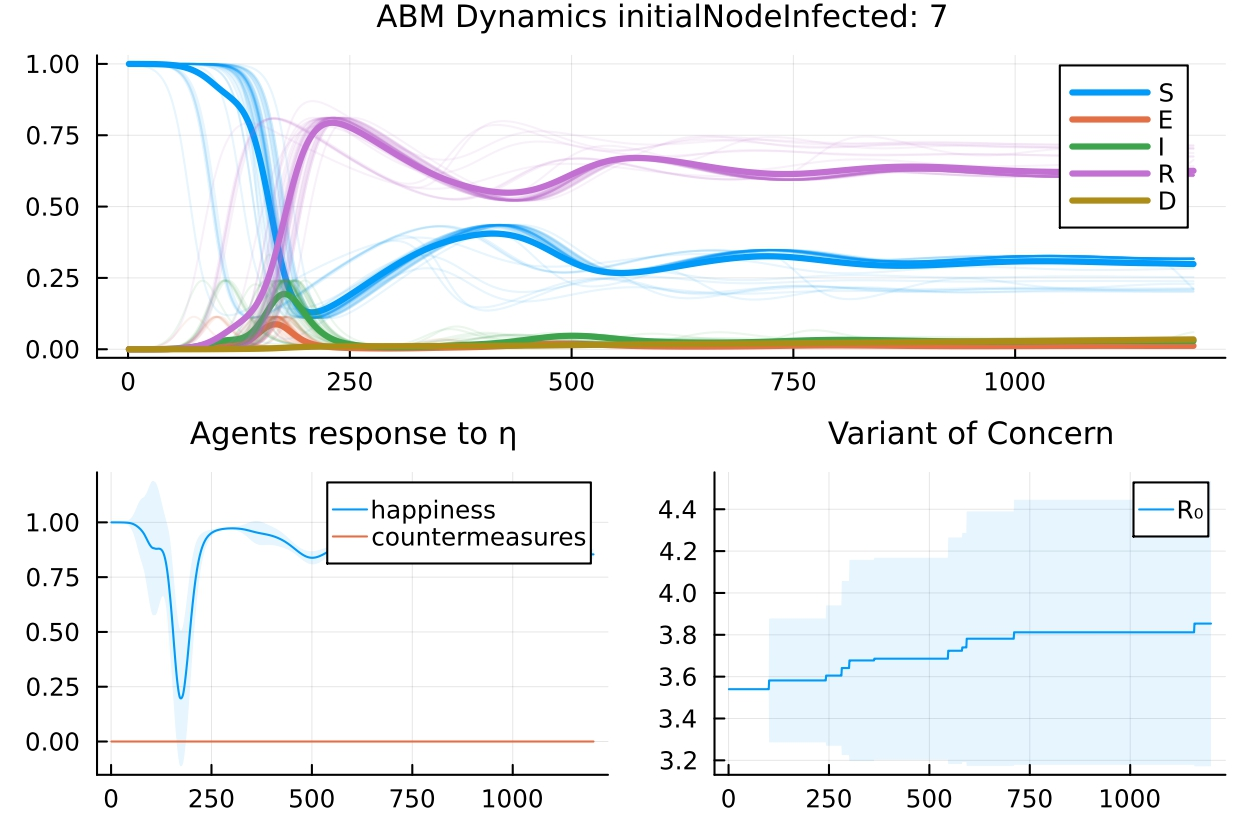
\includegraphics[width=\textwidth]{img/SocialNetworkABM_3_II.jpg}
		\caption{Grafico per la comparazione sul numero di nodi infetti di partenza. Numero nodi infetti iniziali 7}
		\label{fig:comparison_init_node_inf_7}
	\end{subfigure}
	\hfill
	\begin{subfigure}[b]{0.45\textwidth}
		\centering
		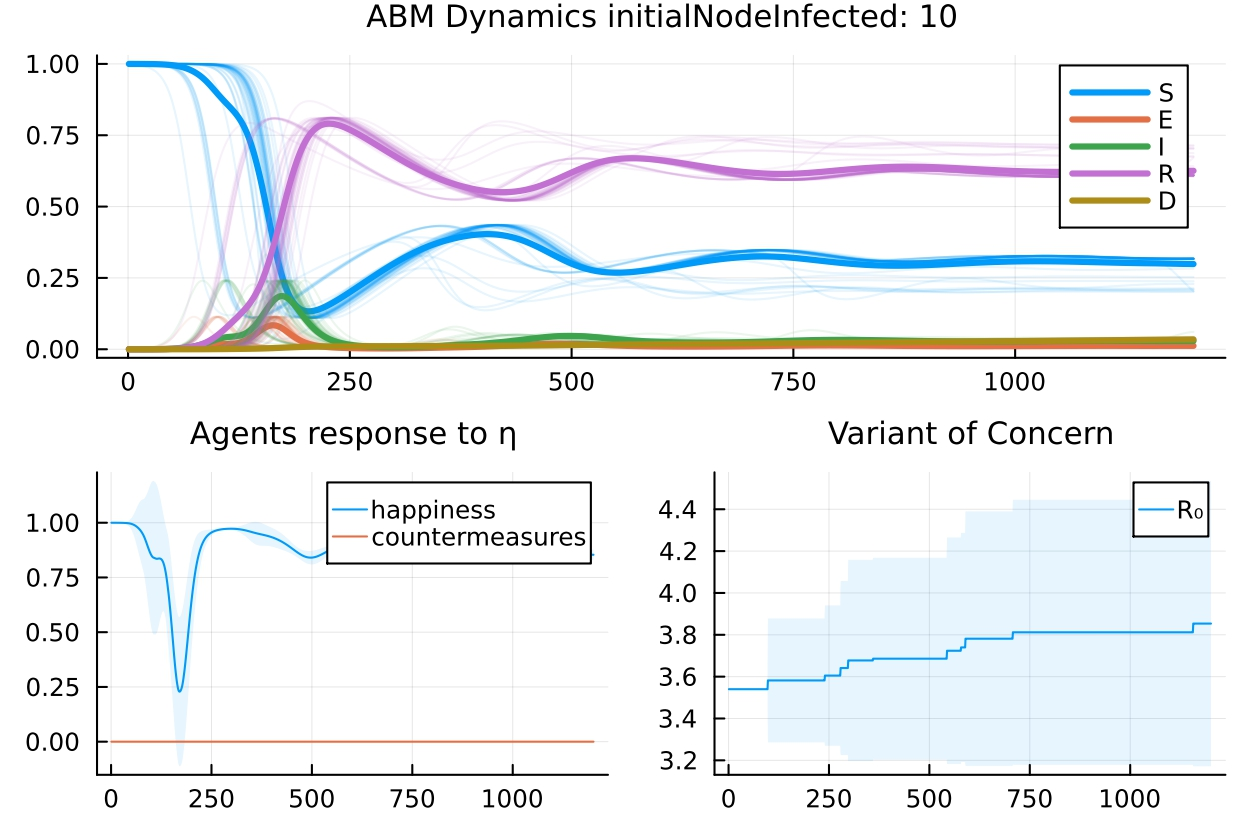
\includegraphics[width=\textwidth]{img/SocialNetworkABM_4_II.jpg}
		\caption{Grafico per la comparazione sul numero di nodi infetti di partenza. Numero nodi infetti iniziali 10}
		\label{fig:comparison_init_node_inf_10}
	\end{subfigure}
\end{figure}

In definitiva, questo risultato conferma la validità delle dinamiche 
epidemiologiche incorporate nel modello e suggerisce che il modello sia 
in grado di riflettere realisticamente l'effetto del numero iniziale di 
infetti sulla diffusione della pandemia, come si verifica anche nella 
realtà.
\newpage

\subsection{Analisi del Comportamento in Base al Tasso di Migrazione}

L'analisi condotta ha esplorato l'influenza del tasso di migrazione sul 
comportamento del modello. I risultati hanno evidenziato che un tasso di 
migrazione più elevato ha generato un picco di individui infetti più alto, 
e ciò è avvenuto in un periodo di tempo più breve rispetto ai casi in cui 
il tasso di migrazione era più basso.

Questo risultato è coerente con le conoscenze consolidate riguardo 
all'effetto della mobilità sulla diffusione delle malattie infettive. 
Infatti, un aumento del tasso di migrazione implica un maggiore movimento 
delle persone tra i nodi del grafo (rappresentanti aree geografiche o 
comunità), il che può facilitare la trasmissione del virus da un luogo 
all'altro. Di conseguenza, si verifica un aumento più rapido e 
pronunciato nel numero di individui infetti, portando a un picco più 
alto in un tempo più breve.

\begin{figure}[!hb]
	\centering
	\begin{subfigure}[b]{0.45\textwidth}
		\centering
		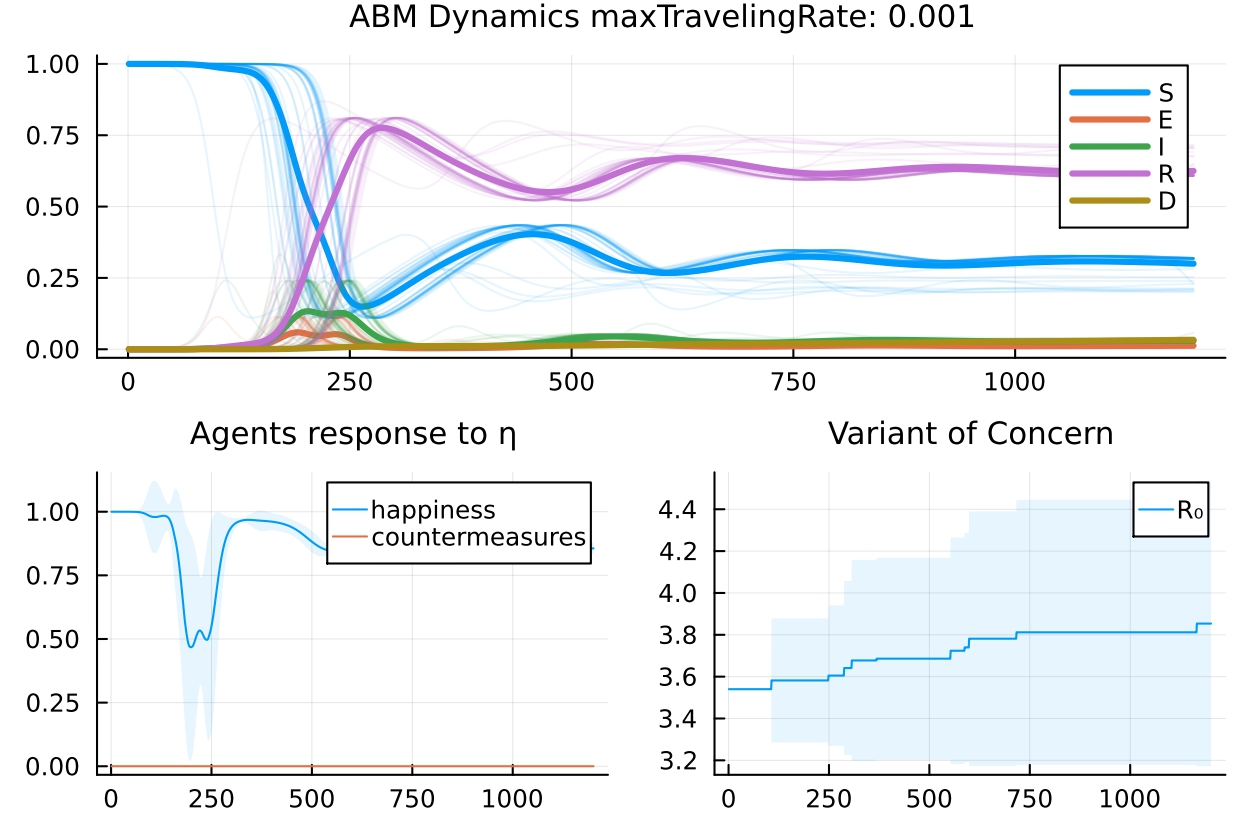
\includegraphics[width=\textwidth]{img/SocialNetworkABM_1_MTR.jpg}
		\caption{Grafico per la comparazione sul valore di migrazione. Valore di 0.001}
		\label{fig:comparison_maxTravelingRate_low}
	\end{subfigure}
	\hfill
	\begin{subfigure}[b]{0.45\textwidth}
		\centering
		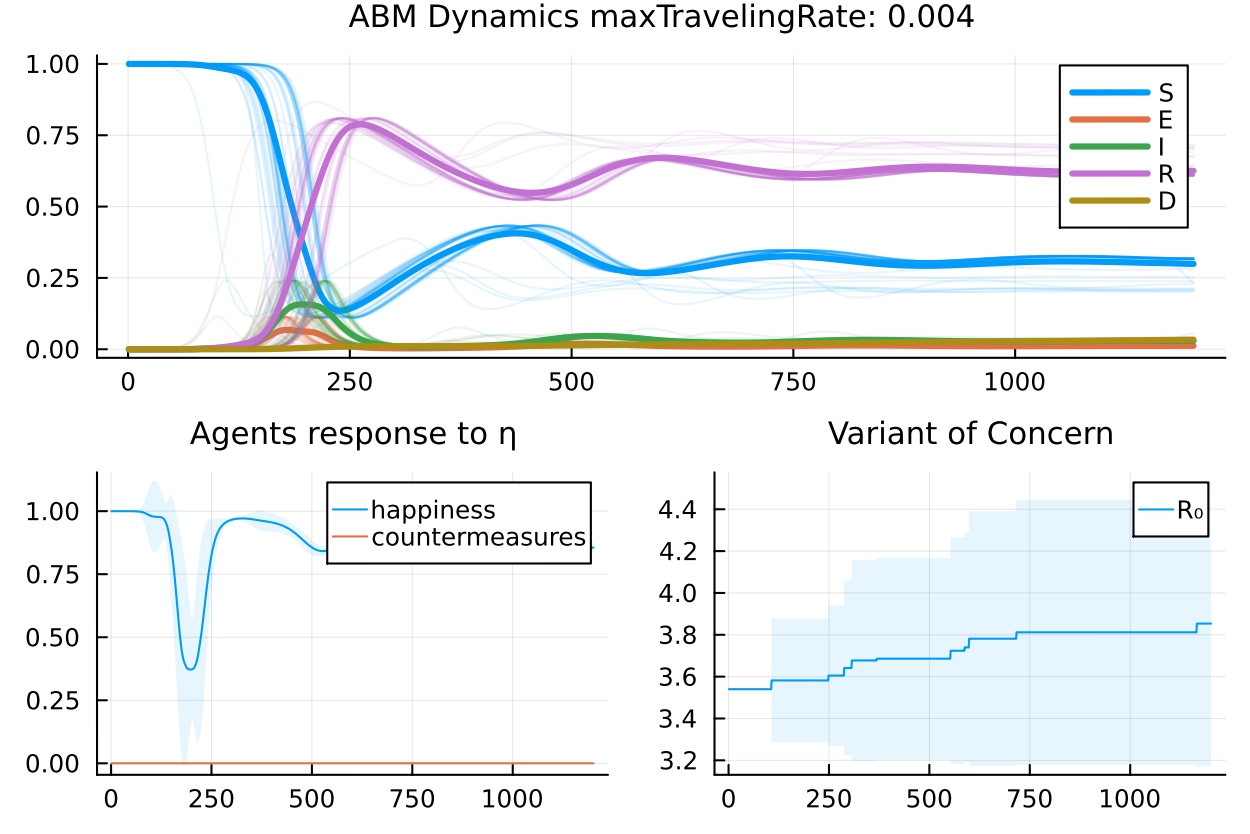
\includegraphics[width=\textwidth]{img/SocialNetworkABM_2_MTR.jpg}
		\caption{Grafico per la comparazione sul valore di migrazione. Valore di 0.004}
		\label{fig:comparison_maxTravelingRate_midl}
	\end{subfigure}
	\hfill
	\begin{subfigure}[b]{0.45\textwidth}
		\centering
		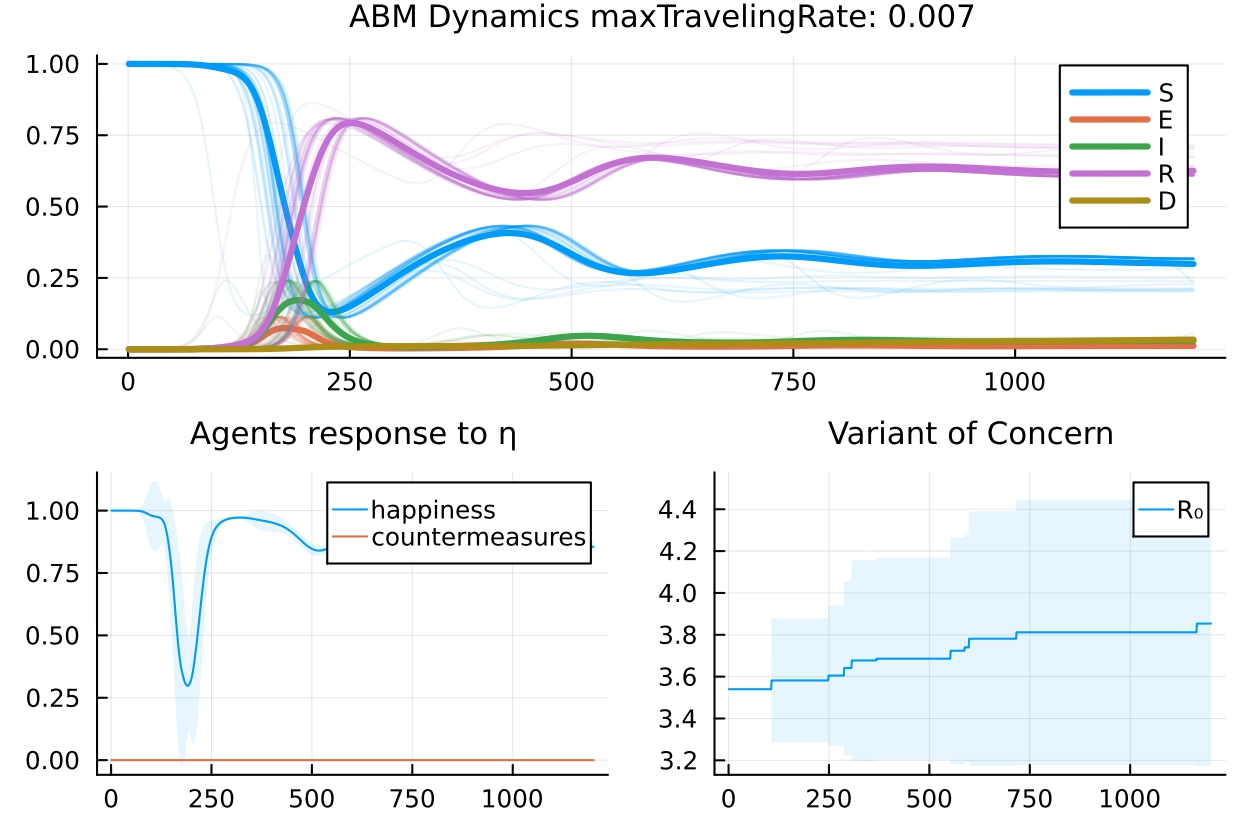
\includegraphics[width=\textwidth]{img/SocialNetworkABM_3_MTR.jpg}
		\caption{Grafico per la comparazione sul valore di migrazione. Valore di 0.007}
		\label{fig:comparison_maxTravelingRate_midh}
	\end{subfigure}
	\hfill
	\begin{subfigure}[b]{0.45\textwidth}
		\centering
		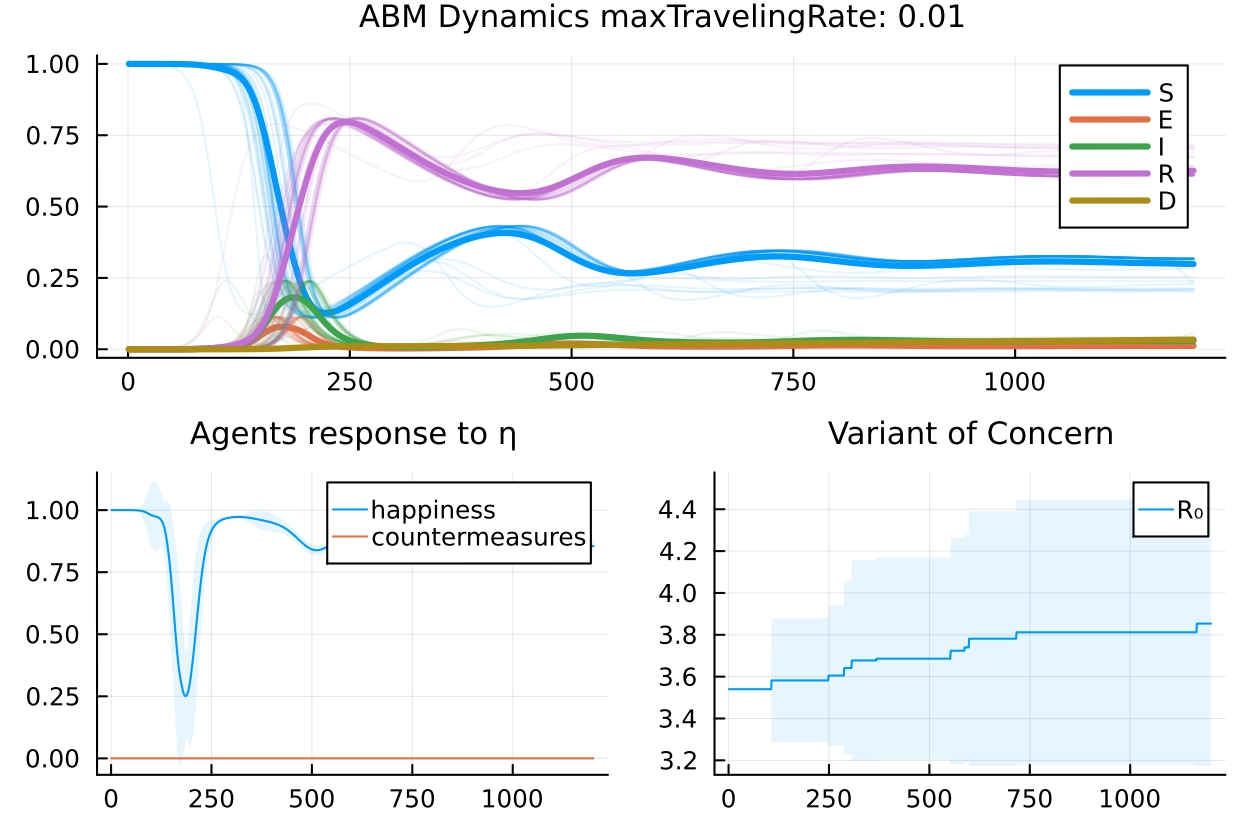
\includegraphics[width=\textwidth]{img/SocialNetworkABM_4_MTR.jpg}
		\caption{Grafico per la comparazione sul valore di migrazione. Valore di 0.01}
		\label{fig:comparison_maxTravelingRate_high}
	\end{subfigure}
\end{figure}

Questi risultati sottolineano l'importanza della mobilità e dei flussi 
di persone nel contesto della diffusione di malattie infettive, come le 
pandemie. Essi sottolineano anche la capacità del modello di catturare 
in modo realistico queste dinamiche epidemiologiche, consentendo una 
valutazione approfondita degli effetti del tasso di migrazione sul 
comportamento del sistema.
\newpage

\subsection{Analisi del Comportamento in Base al Numero di Nodi della Rete}

L'analisi condotta ha investigato come il numero di nodi nella rete 
influenzi il comportamento complessivo del modello. 
Dai risultati è emerso che un numero maggiore di nodi nella rete ha 
comportato una diffusione più lenta della pandemia e ha generato picchi 
meno ripidi ma più prolungati nel tempo.

Questo risultato è influenzato da diversi fattori, tra cui la 
topologia delle connessioni tra i nodi e la posizione del focolaio 
iniziale della pandemia. Quando ci sono più nodi nella rete, 
la trasmissione del virus può richiedere più tempo per propagarsi 
attraverso l'intera popolazione, dato che ci sono più "tappe" attraverso 
cui deve passare. Inoltre, la posizione iniziale del focolaio può 
influenzare la velocità di diffusione, in quanto i nodi vicini al 
focolaio avranno una probabilità maggiore di essere infettati 
inizialmente rispetto ai nodi più lontani.

Di conseguenza, si osserva una diffusione più graduale della pandemia 
nel corso del tempo, con picchi meno ripidi ma più prolungati. 
Questo risultato è coerente con l'effetto della dimensione della 
popolazione e della struttura della rete sulla diffusione di malattie 
infettive.

\begin{figure}[!hb]
	\centering
	\begin{subfigure}[b]{0.45\textwidth}
		\centering
		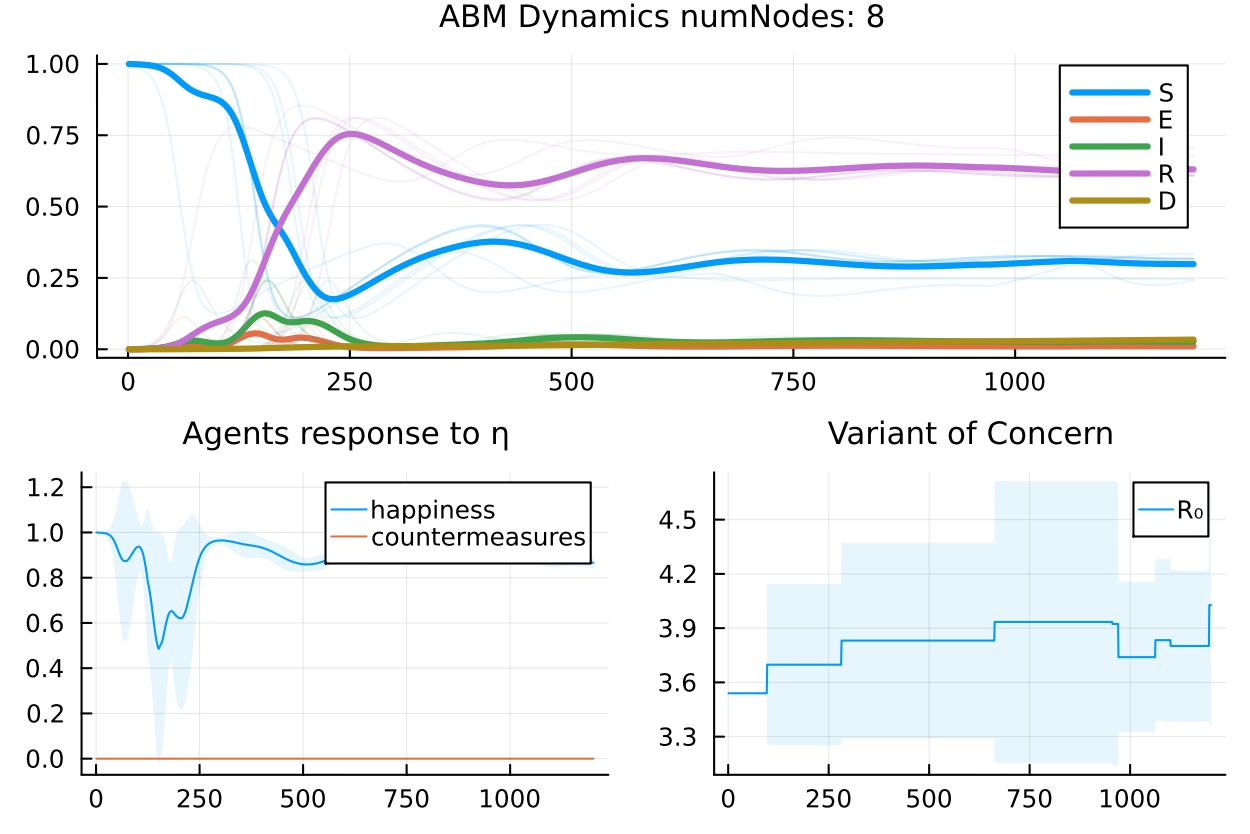
\includegraphics[width=\textwidth]{img/SocialNetworkABM_1_NN.jpg}
		\caption{Grafico per la comparazione sul numero di nodi della rete. Numero nodi 8}
		\label{fig:comparison_numberOfNodes_8}
	\end{subfigure}
	\hfill
	\begin{subfigure}[b]{0.45\textwidth}
		\centering
		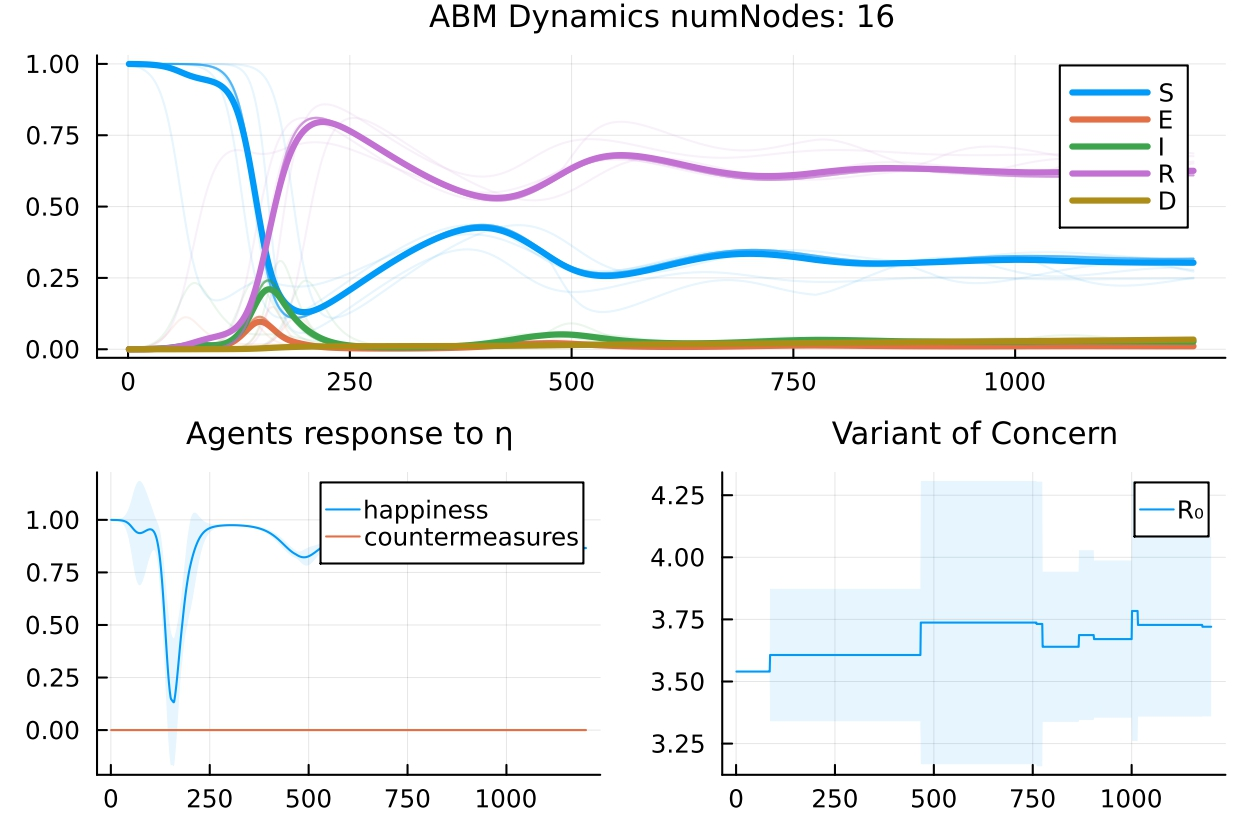
\includegraphics[width=\textwidth]{img/SocialNetworkABM_2_NN.jpg}
		\caption{Grafico per la comparazione sul numero di nodi della rete. Numero nodi 16}
		\label{fig:comparison_numberOfNodes_16}
	\end{subfigure}
	\hfill
	\begin{subfigure}[b]{0.45\textwidth}
		\centering
		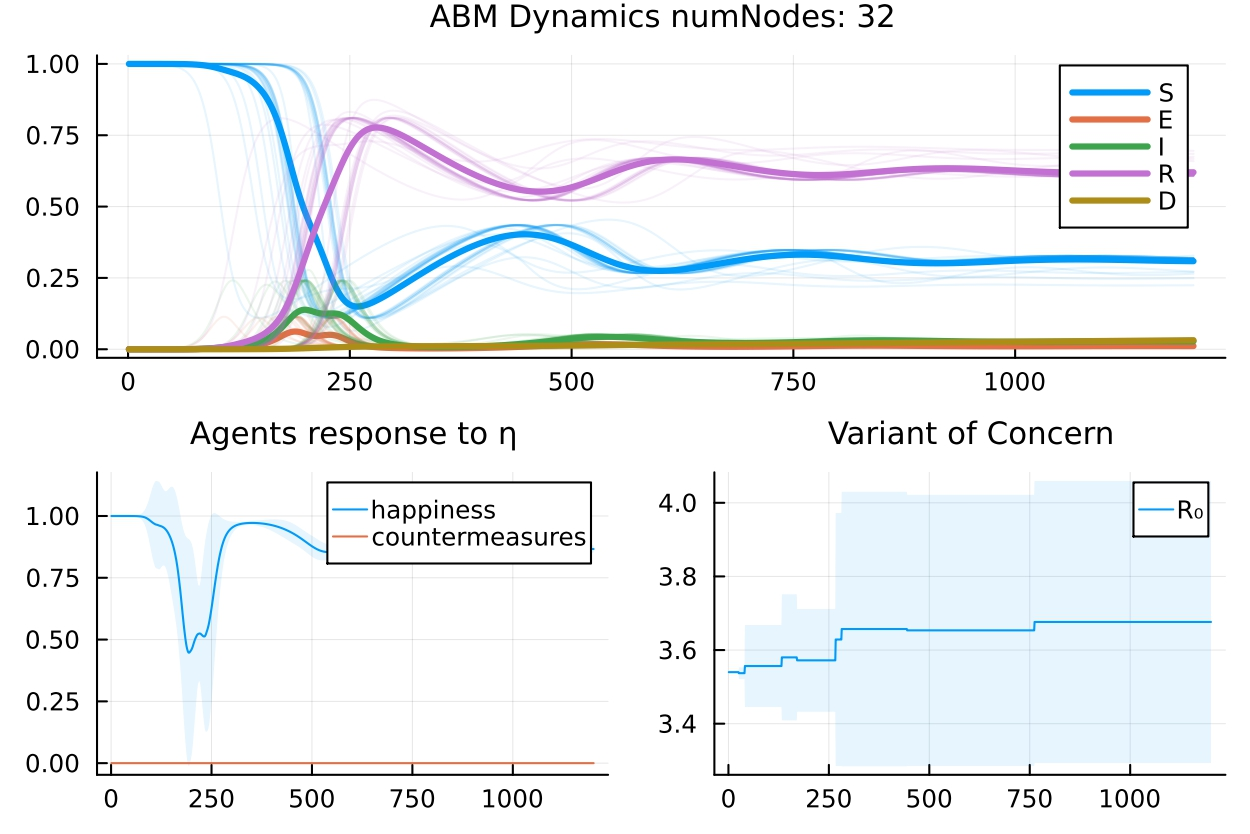
\includegraphics[width=\textwidth]{img/SocialNetworkABM_3_NN.jpg}
		\caption{Grafico per la comparazione sul numero di nodi della rete. Numero nodi 32}
		\label{fig:comparison_numberOfNodes_32}
	\end{subfigure}
	\hfill
	\begin{subfigure}[b]{0.45\textwidth}
		\centering
		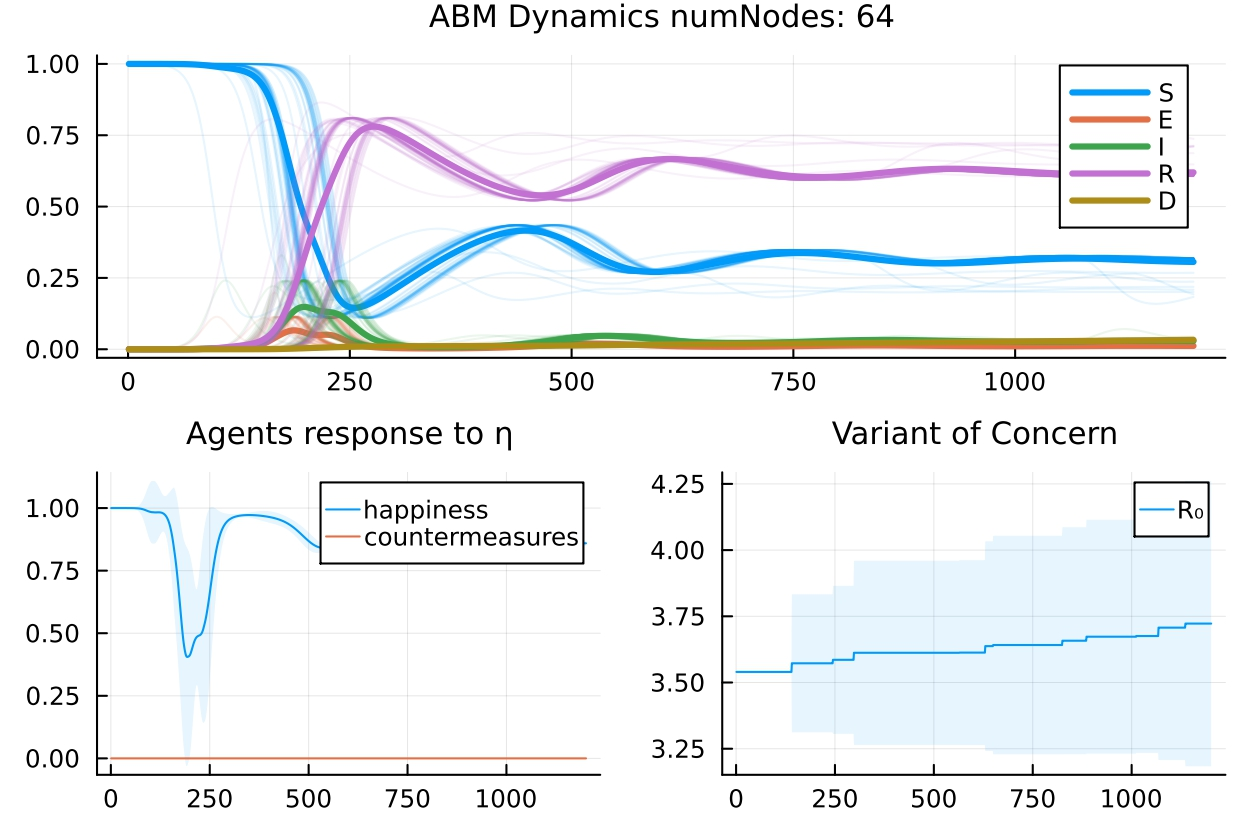
\includegraphics[width=\textwidth]{img/SocialNetworkABM_4_NN.jpg}
		\caption{Grafico per la comparazione sul numero di nodi della rete. Numero nodi 64}
		\label{fig:comparison_numberOfNodes_64}
	\end{subfigure}
\end{figure}

In sintesi, l'analisi ha dimostrato come il numero di nodi nella rete, 
insieme a variabili come la topologia delle connessioni e la posizione 
iniziale del focolaio, possa influenzare in modo significativo le 
dinamiche della pandemia e i profili temporali di infezione.
\newpage

\subsection{Analisi del Comportamento in Base alla Copertura della Rete}

L'analisi condotta ha esaminato l'effetto della copertura della rete, 
rappresentata dal numero di archi, sul comportamento del modello. 
Dai risultati è emerso che una copertura bassa, ovvero un numero 
limitato di connessioni tra i nodi del grafo, ha comportato un 
rallentamento significativo nella diffusione del virus, analogamente 
all'effetto di misure di contenimento come il lockdown. 
Questo risultato è coerente con l'importanza della mobilità nella 
diffusione delle malattie infettive e sottolinea il ruolo cruciale 
delle misure di contenimento nel limitare la propagazione del virus.

Inoltre, è stato osservato che il numero di Varianti di Interesse 
(VOC) tende ad aumentare con il numero di nodi nella rete. 
Questo suggerisce che in una popolazione più ampia, c'è una maggiore 
probabilità di emergere nuove mutazioni. Tuttavia, è interessante 
notare che la presenza di una bassa copertura, cioè una limitata 
interconnessione tra i nodi, può limitare la diffusione delle varianti 
stesse, poiché la trasmissione tra gli individui è ridotta.

\begin{figure}[!hb]
	\centering
	\begin{subfigure}[b]{0.3\textwidth}
		\centering
		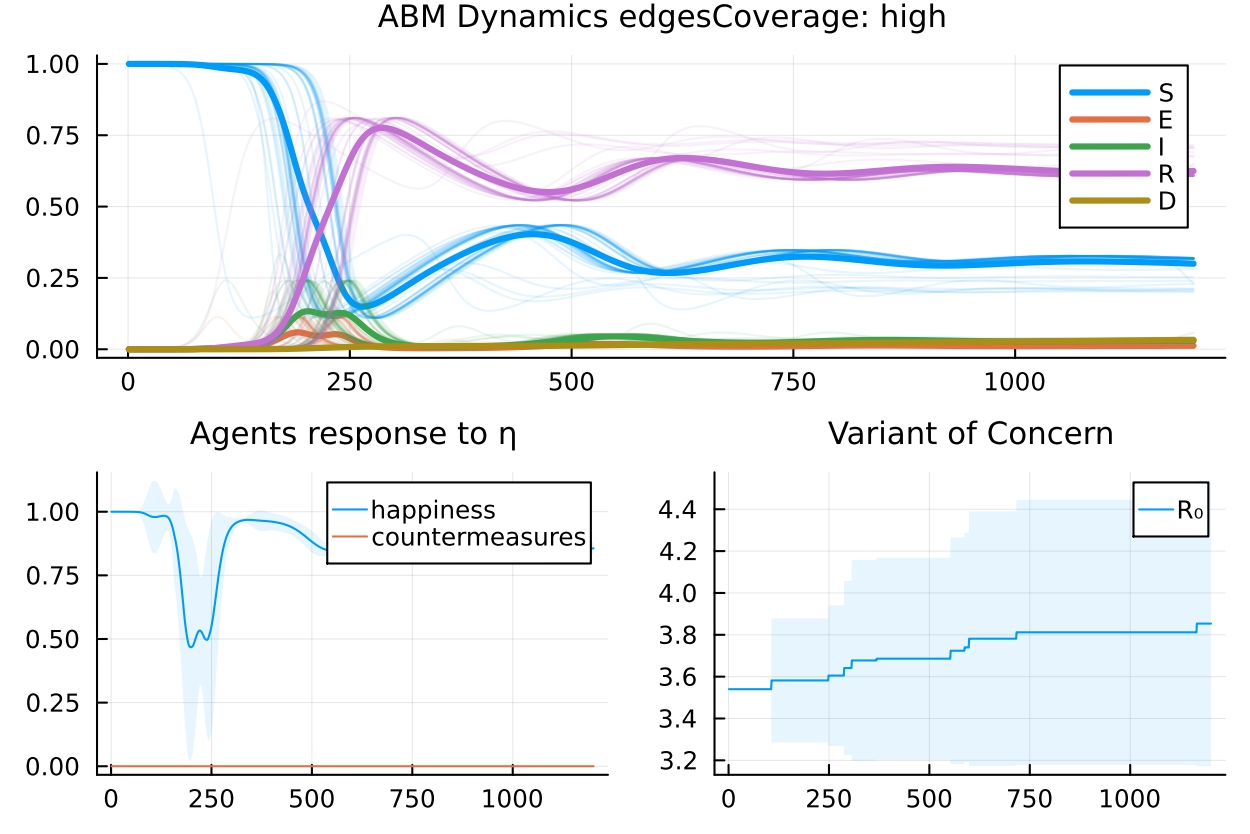
\includegraphics[width=\textwidth]{img/SocialNetworkABM_1_EC.jpg}
		\caption{Grafico per la comparazione sulla copertura della rete. Copertura alta}
		\label{fig:comparison_highCoverage}
	\end{subfigure}
	\hfill
	\begin{subfigure}[b]{0.3\textwidth}
		\centering
		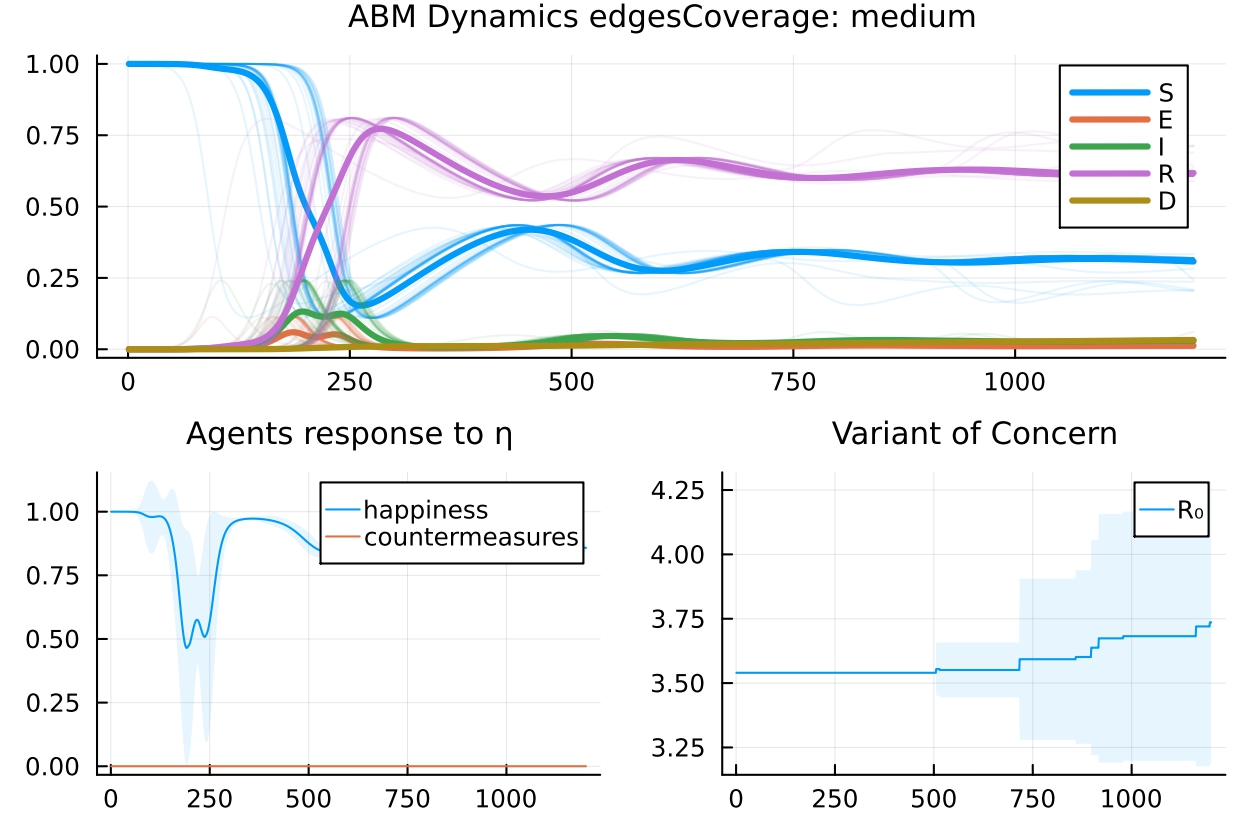
\includegraphics[width=\textwidth]{img/SocialNetworkABM_2_EC.jpg}
		\caption{Grafico per la comparazione sulla copertura della rete. Copertura media}
		\label{fig:comparison_mediumCoverage}
	\end{subfigure}
	\hfill
	\begin{subfigure}[b]{0.3\textwidth}
		\centering
		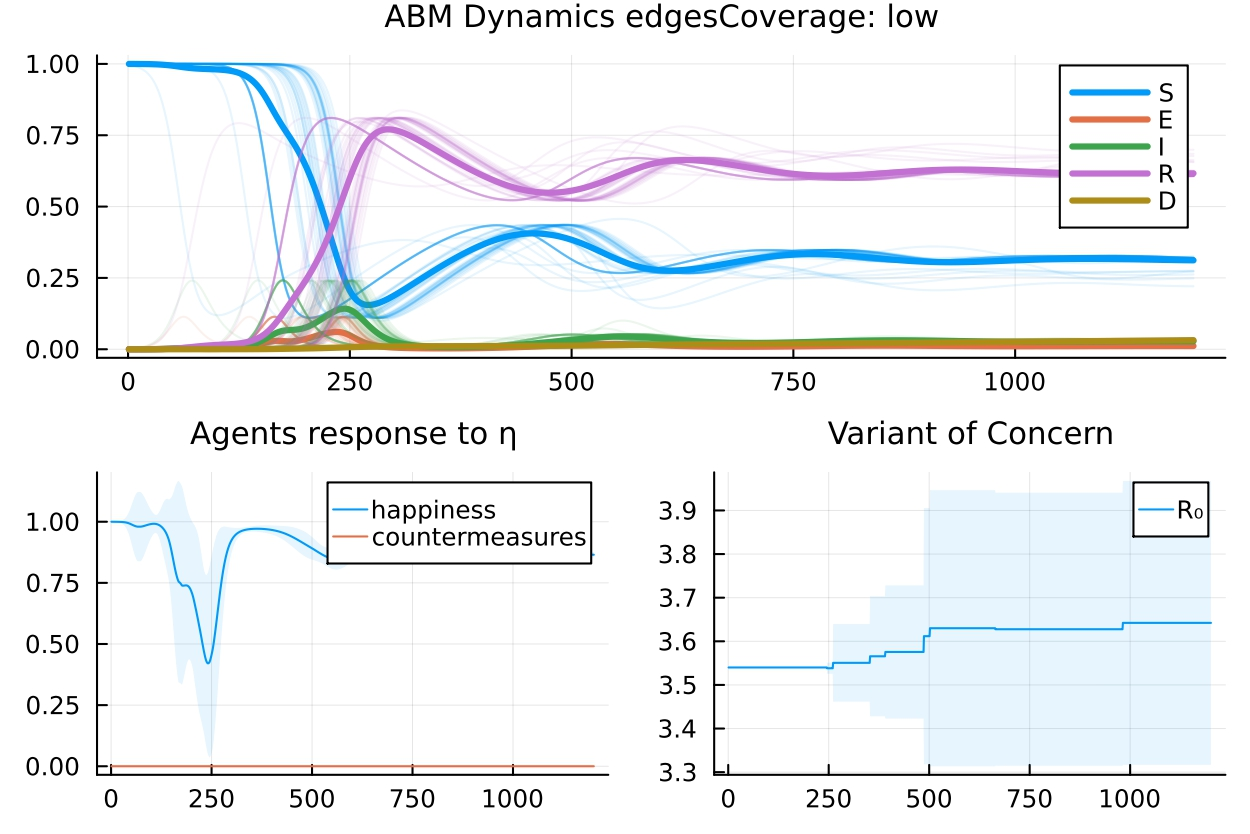
\includegraphics[width=\textwidth]{img/SocialNetworkABM_3_EC.jpg}
		\caption{Grafico per la comparazione sulla copertura della rete. Copertura bassa}
		\label{fig:comparison_lowCoverage}
	\end{subfigure}
\end{figure}

In sintesi, l'analisi ha rivelato come vari parametri e condizioni, 
tra cui la copertura della rete, la mobilità, le misure di contenimento 
e il numero di nodi, possono influenzare in modo significativo il 
comportamento del modello epidemiologico. Questi risultati forniscono 
importanti informazioni per la comprensione e la gestione delle epidemie, 
evidenziando l'importanza delle strategie di mitigazione e della 
considerazione della struttura della rete nella prevenzione della 
diffusione del virus.

\subsection{Studio dell'Andamento del Controllore in Relazione all'Intervallo di Intervento}
L'analisi condotta nel presente studio ha investigato l'influenza 
dell'intervallo di intervento del controllore in relazione al controllo 
della pandemia e all'andamento della curva di "happiness". I risultati 
ottenuti hanno rivelato che un incremento nel valore associato 
all'intervallo di intervento provoca un notevole sbilanciamento nella 
curva di felicità ("happiness") e, in generale, comporta un repentino 
aumento nei valori associati alle contromisure adottate.

Tale andamento, coerente e previsto, può essere spiegato dalla 
complessità intrinseca nel formulare contromisure a lungo termine 
rispetto a quelle a breve termine, oltre al fatto che le prime 
comportano costi maggiori. È interessante notare che l'andamento delle 
curve, come mostrato nelle Figure \ref{fig:comparison_dt_21} e 
\ref{fig:comparison_dt_28}, ha rivelato comportamenti inaspettati che 
non erano stati previsti inizialmente. Questo comportamento inusuale è 
probabilmente riconducibile alla definizione della funzione di loss, 
come illustrato nella Figura \ref{fig:lossFunction}, e alle successive 
iterazioni di addestramento della rete.

In conclusione, dai risultati ottenuti emerge che attualmente le curve 
più affidabili sono quelle associate a un intervallo di intervento più 
breve. Tuttavia, è importante notare che non sono stati esplorati 
intervalli troppo granulari a causa del loro significativo impatto 
sulle prestazioni del sistema e, soprattutto, della loro limitata 
rappresentatività nella realtà.

\begin{figure}[!hb]
	\centering
	\begin{subfigure}[b]{0.45\textwidth}
		\centering
		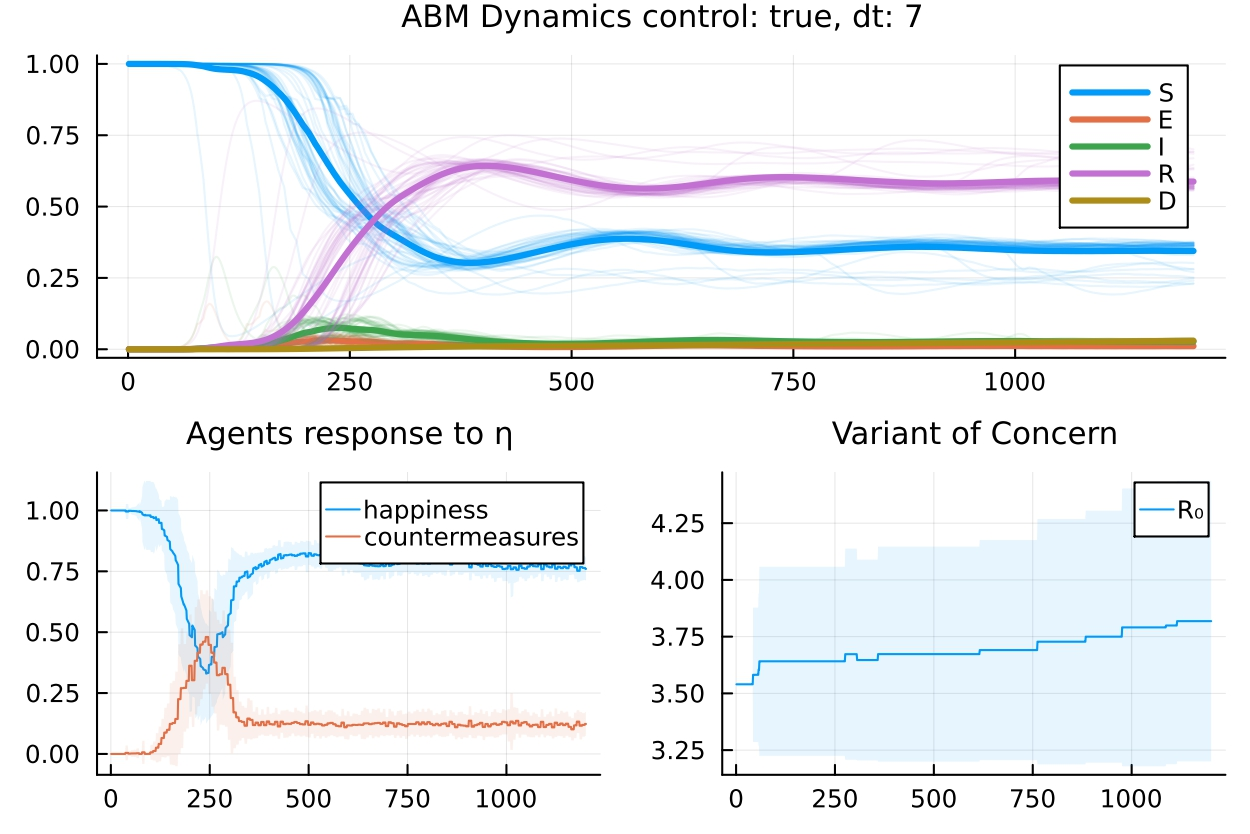
\includegraphics[width=\textwidth]{img/SocialNetworkABM_1_DT.jpg}
		\caption{Grafico per la comparazione sul valore dell'intervallo di intervento del controllore. Valore 7 step}
		\label{fig:comparison_dt_7}
	\end{subfigure}
	\hfill
	\begin{subfigure}[b]{0.45\textwidth}
		\centering
		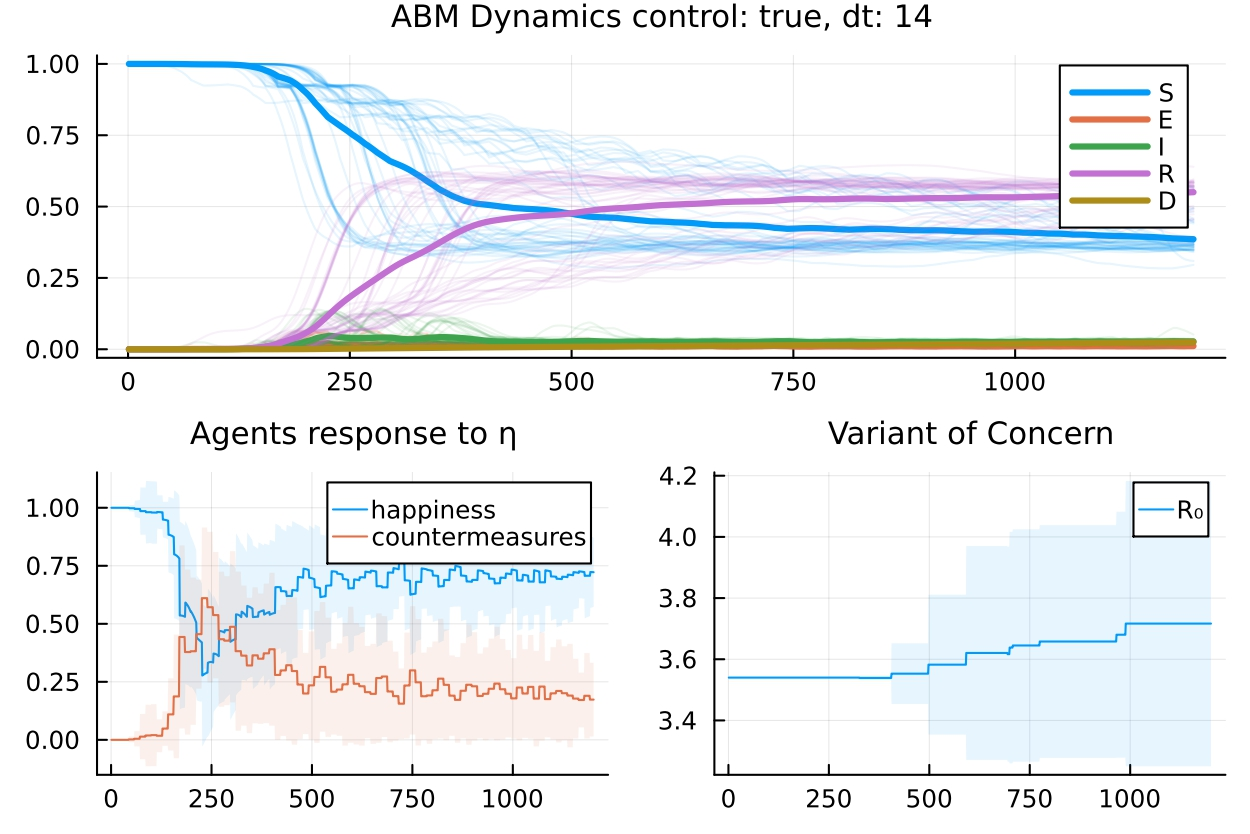
\includegraphics[width=\textwidth]{img/SocialNetworkABM_2_DT.jpg}
		\caption{Grafico per la comparazione sul valore dell'intervallo di intervento del controllore. Valore 14 step}
		\label{fig:comparison_dt_14}
	\end{subfigure}
	\hfill
	\begin{subfigure}[b]{0.45\textwidth}
		\centering
		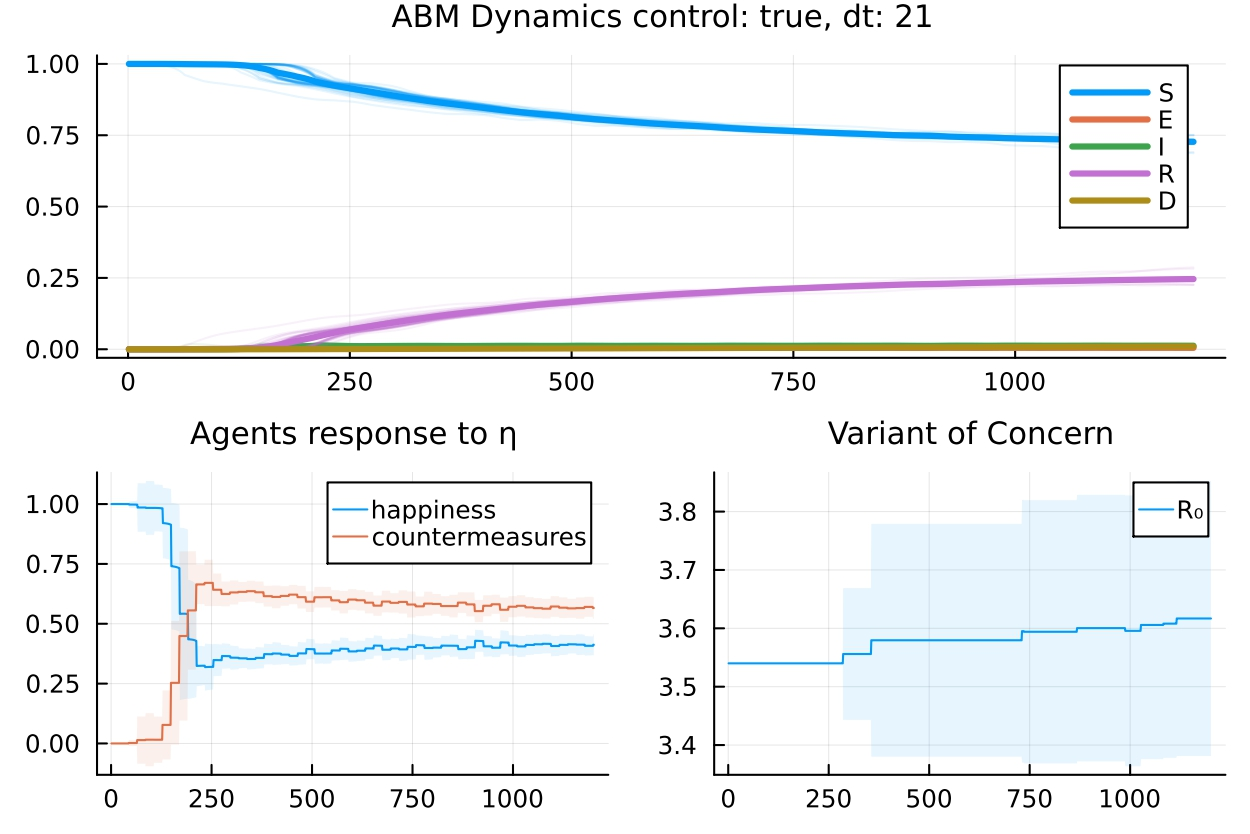
\includegraphics[width=\textwidth]{img/SocialNetworkABM_3_DT.jpg}
		\caption{Grafico per la comparazione sul valore dell'intervallo di intervento del controllore. Valore 21 step}
		\label{fig:comparison_dt_21}
	\end{subfigure}
	\hfill
	\begin{subfigure}[b]{0.45\textwidth}
		\centering
		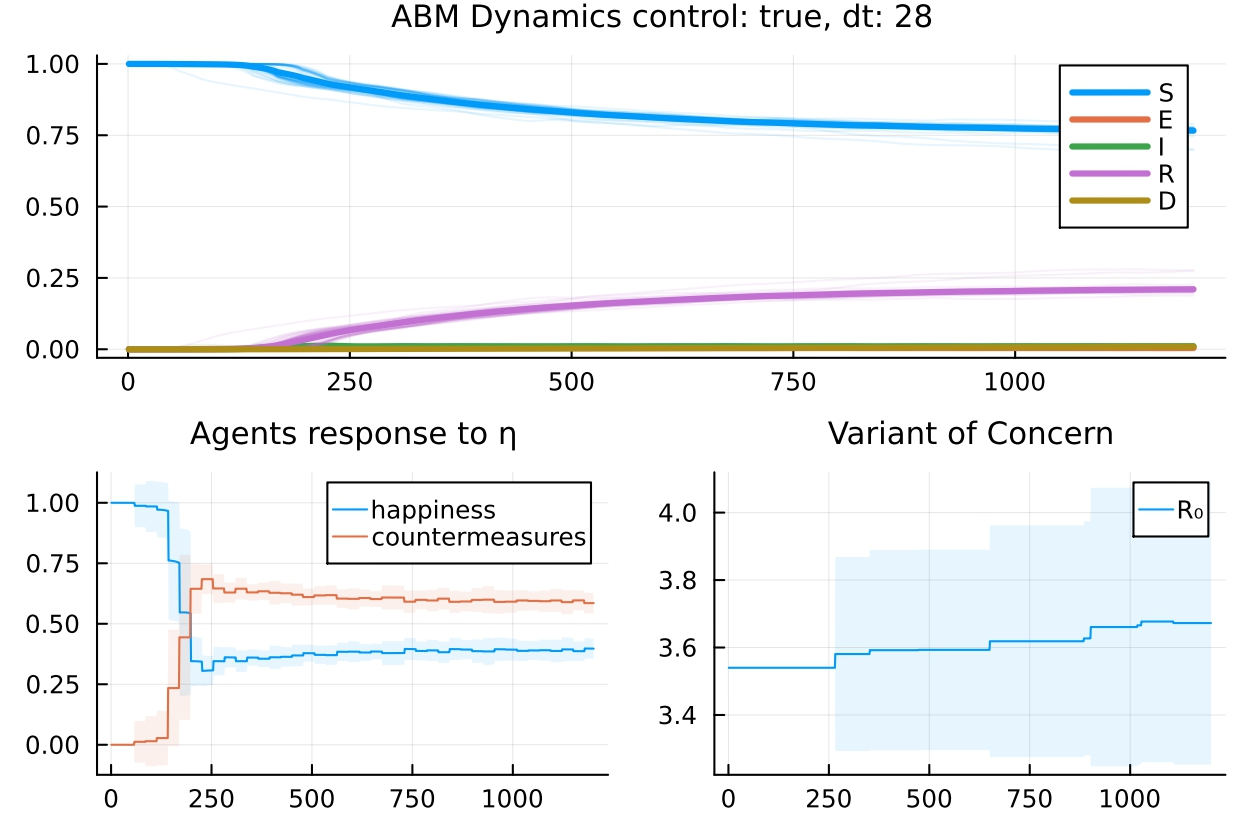
\includegraphics[width=\textwidth]{img/SocialNetworkABM_4_DT.jpg}
		\caption{Grafico per la comparazione sul valore dell'intervallo di intervento del controllore. Valore 28 step}
		\label{fig:comparison_dt_28}
	\end{subfigure}
\end{figure}

\subsection{Studio dell'Andamento del Controllore in Relazione all'Intervallo di Tolleranza}
L'analisi condotta nel corso di questa indagine ha approfondito 
l'influenza dell'intervallo di tolleranza del controllore in relazione 
al controllo della pandemia e all'andamento della curva di "happiness". 
Dalla nostra analisi emerge chiaramente che il valore di tolleranza del 
controllore svolge un ruolo cruciale soprattutto durante il picco pandemico.

Tuttavia, è degno di nota che un valore di tolleranza estremamente 
elevato incide in maniera significativa sull'andamento complessivo del 
modello, ritardando l'attuazione delle contromisure e costringendo il 
controllore ad adottare un comportamento molto più drastico rispetto alle 
aspettative.

È fondamentale sottolineare che tali risultati sono ampiamente 
condizionati dal numero di individui presenti in ciascun nodo del modello. 
Il test è stato condotto su un modello composto da cinquanta nodi, ognuno 
dei quali ospitava un numero di individui distribuiti secondo una 
distribuzione esponenziale con un parametro medio pari a 10.000. 
Questo implica che l'interpretazione dei risultati deve essere 
attentamente valutata tenendo conto del valore medio di popolazione 
all'interno del modello.

Evidentemente, è cruciale riconoscere come l'aumento del valore di 
popolazione generi risultati differenti. In scenari caratterizzati da 
valori di popolazione medio relativamente bassi, è possibile adottare 
una soglia di tolleranza più elevata, mentre in situazioni in cui la 
popolazione è notevolmente elevata, diventa necessario aumentare la 
tolleranza al fine di garantire un adeguato controllo.

In conclusione, l'analisi effettuata dimostra che l'intervallo di 
tolleranza del controllore rappresenta un fattore chiave nella gestione 
della pandemia e dell'andamento della "happiness". La sua ottimizzazione 
deve essere attentamente bilanciata in base al contesto specifico, inclusi 
il numero di individui e le dinamiche di popolazione, al fine di garantire 
un controllo efficace e tempestivo della pandemia.

\begin{figure}[!hb]
	\centering
	\begin{subfigure}[b]{0.45\textwidth}
		\centering
		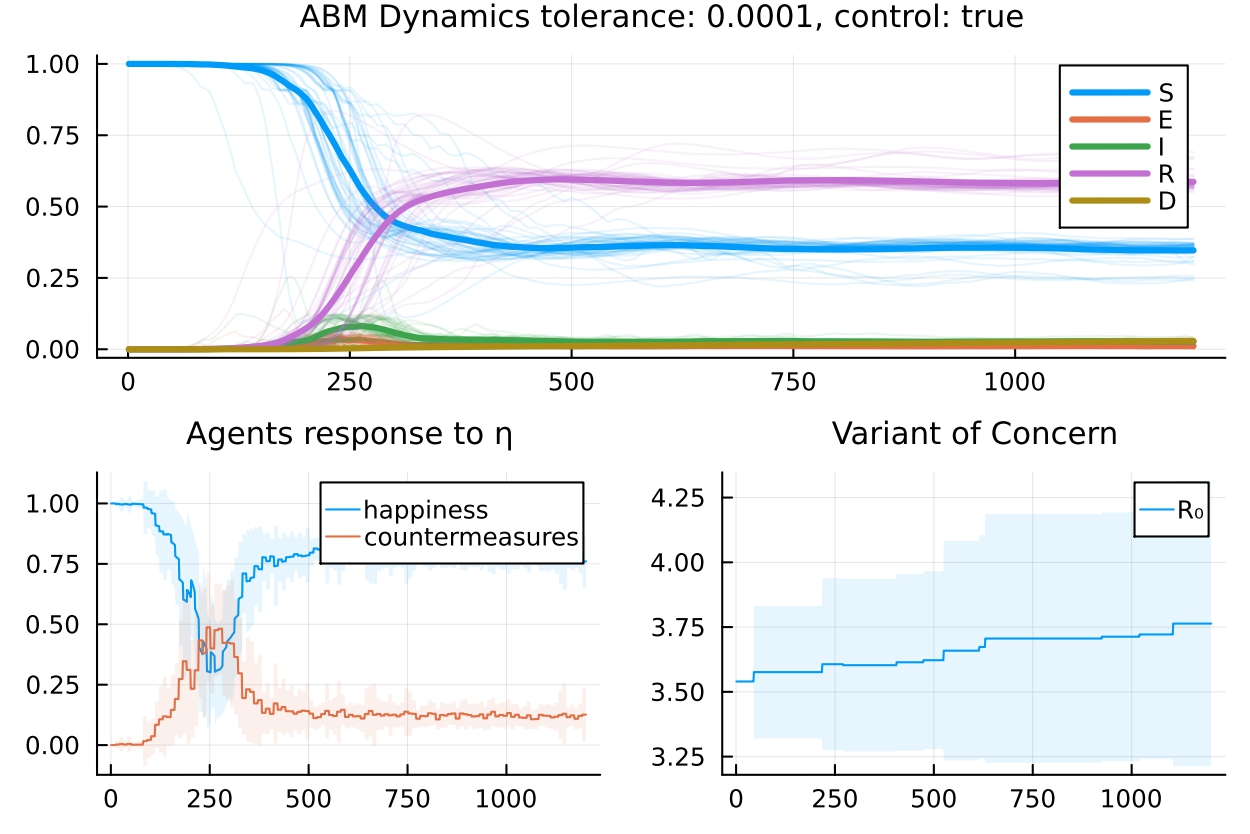
\includegraphics[width=\textwidth]{img/SocialNetworkABM_1_TOL.jpg}
		\caption{Grafico per la comparazione sul valore di attivazione del controllore. Valore di tolleranza 0.0001}
		\label{fig:comparison_tol_1e-4}
	\end{subfigure}
	\hfill
	\begin{subfigure}[b]{0.45\textwidth}
		\centering
		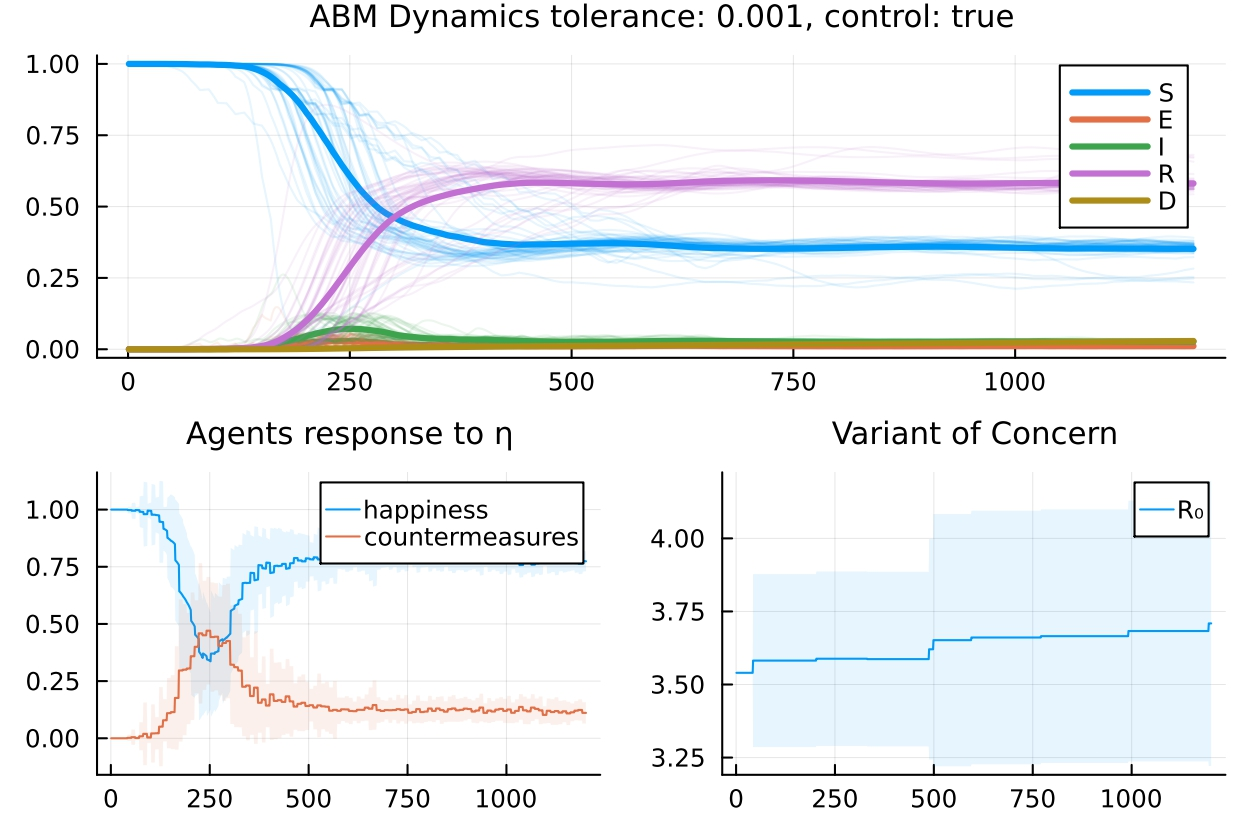
\includegraphics[width=\textwidth]{img/SocialNetworkABM_2_TOL.jpg}
		\caption{Grafico per la comparazione sul valore di attivazione del controllore. Valore di tolleranza 0.001}
		\label{fig:comparison_tol_1e-3}
	\end{subfigure}
	\hfill
	\begin{subfigure}[b]{0.45\textwidth}
		\centering
		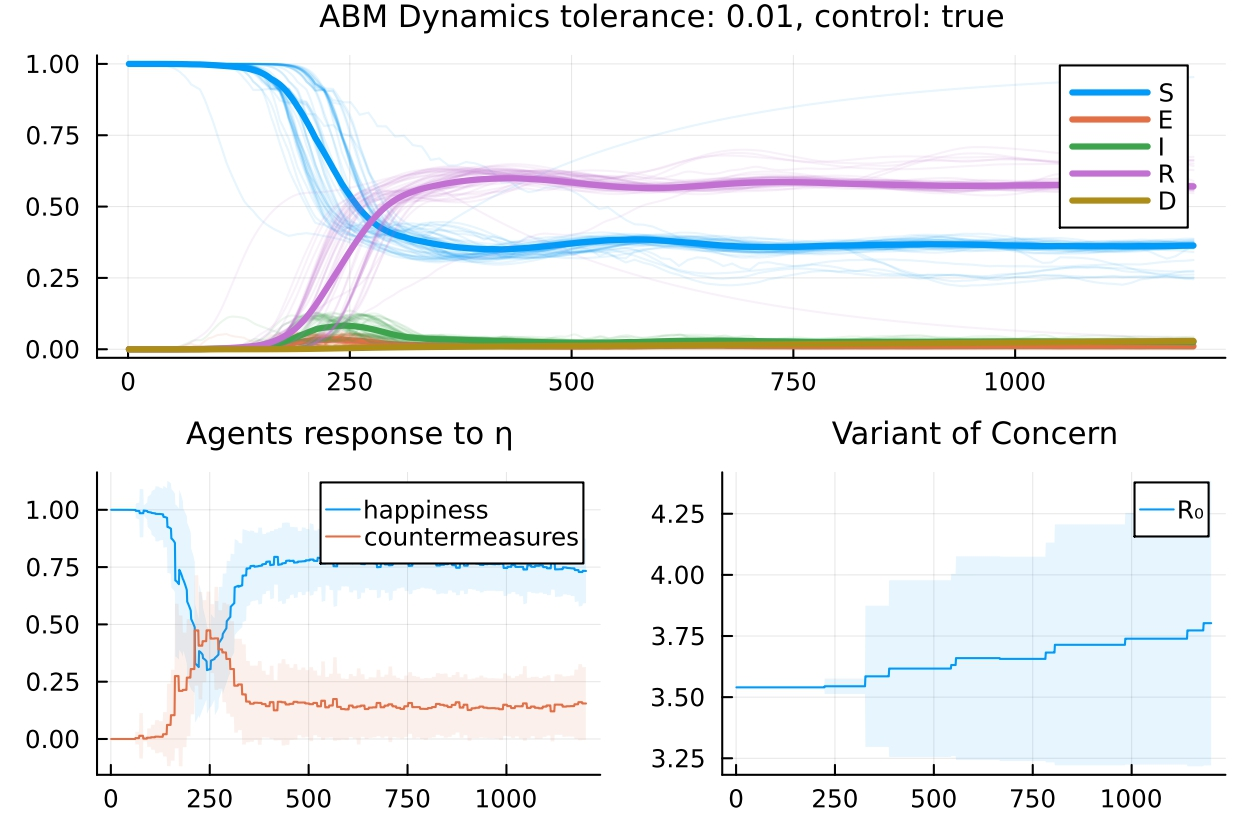
\includegraphics[width=\textwidth]{img/SocialNetworkABM_3_TOL.jpg}
		\caption{Grafico per la comparazione sul valore di attivazione del controllore. Valore di tolleranza 0.01}
		\label{fig:comparison_tol_1e-2}
	\end{subfigure}
	\hfill
	\begin{subfigure}[b]{0.45\textwidth}
		\centering
		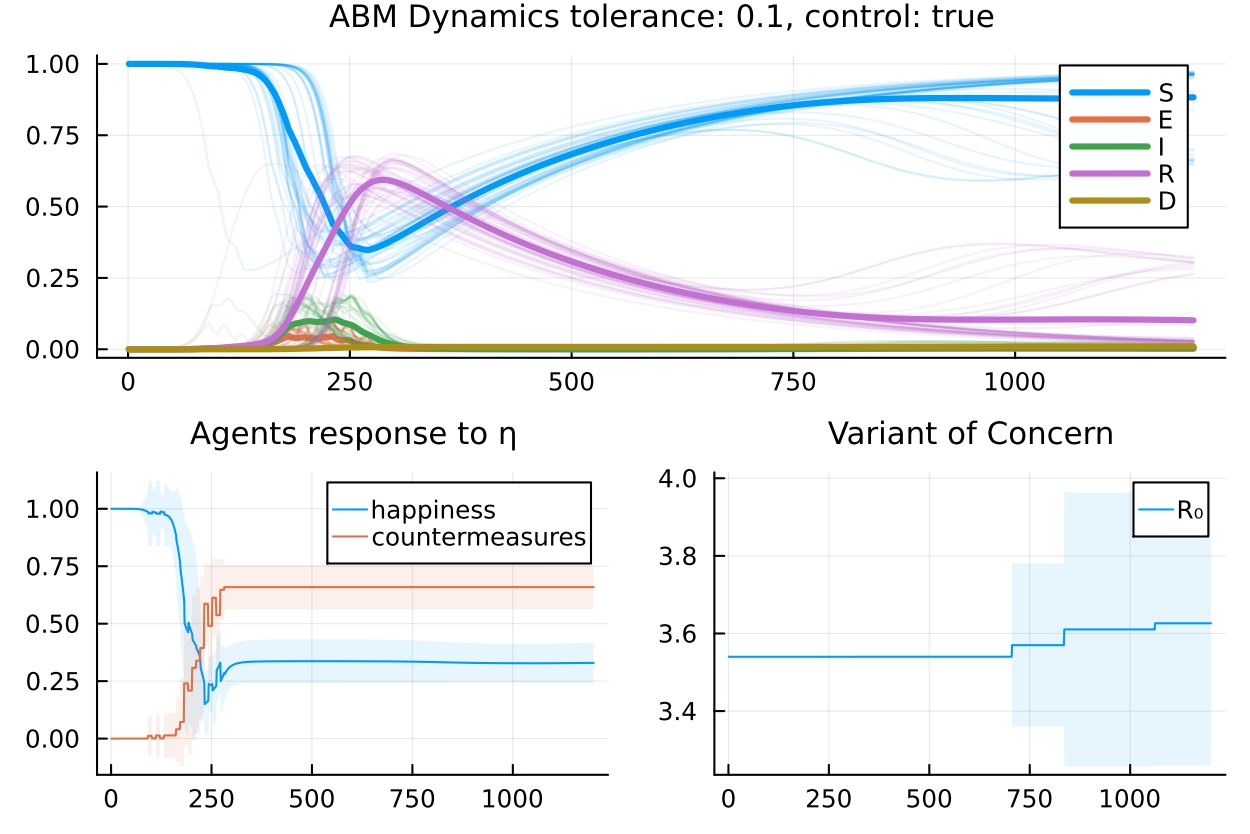
\includegraphics[width=\textwidth]{img/SocialNetworkABM_4_TOL.jpg}
		\caption{Grafico per la comparazione sul valore di attivazione del controllore. Valore di tolleranza 0.1}
		\label{fig:comparison_tol_1e-1}
	\end{subfigure}
\end{figure}

In entrambi i contesti in cui sono stati esaminati e testati alcuni 
parametri fondamentali del controllore, è evidente come la curva di 
"happiness" mostri un comportamento apparentemente opposto rispetto alla 
curva delle contromisure adottate. Questo fenomeno è chiaramente 
attribuibile alla natura estremamente semplicistica con cui è stata 
definita la curva di "happiness", come illustrato nella Figura 
\ref{fig:happinessf}.

Va notato che questa semplificazione nella rappresentazione della 
felicità è stata scelta consapevolmente per scopi specifici di questo 
studio, sebbene sia riconosciuta come irrealistica. Tuttavia, questa 
semplice rappresentazione ha dimostrato di essere adeguata per gli 
obiettivi attuali della ricerca. 

Nonostante l'apparente discrepanza tra i comportamenti delle due curve, 
è importante sottolineare che questa semplificazione sarà oggetto di 
ulteriori raffinamenti in futuro. Tale rifinitura mirerà a renderla più 
realistica e coerente con le dinamiche reali delle emozioni umane e 
delle reazioni della società a situazioni di emergenza.

In conclusione, la discrepanza osservata tra le curve di "happiness" e 
le curve delle contromisure è attribuibile alla semplificazione 
deliberata della curva di "happiness" utilizzata in questo studio. 
Tale semplificazione, sebbene irrealistica, è adeguata agli scopi attuali, 
ma verrà affinata in future ricerche al fine di migliorare la 
rappresentazione delle dinamiche umane in contesti pandemici e di 
emergenza.